\documentclass[11pt,a4paper]{article}

\usepackage[T1]{fontenc}
\usepackage[utf8]{inputenc}
\usepackage[italian]{babel}
\usepackage{amsmath,amssymb}
\usepackage[a4paper,margin=2.5cm]{geometry}
\usepackage{array}
\usepackage{siunitx}
\usepackage{booktabs}
\usepackage{graphicx}
\usepackage{float}
\usepackage{hyperref}

\hypersetup{hidelinks}
\setlength{\parindent}{0pt}
\setlength{\parskip}{4pt}
\allowdisplaybreaks
\graphicspath{{figure/}}
\sisetup{output-decimal-marker={,}, group-separator={\,}, per-mode=symbol,
         exponent-product=\cdot, range-phrase={\text{--}}}

\newcommand{\Ru}{R_1}
\newcommand{\Rd}{R_2}
\newcommand{\uma}{u-a}
\newcommand{\upa}{u+a}
\newcommand{\Me}{M_e}
\newcommand{\Cr}{C_r}

\title{Gasdinamica -- Svolgimento esercizio 2\\[2pt]
\large Condizione al contorno all'uscita di un condotto: Mach imposto e riflessione di un'onda acustica}
\author{}
\date{Prova del 01/03/1970}

\begin{document}
\maketitle

\section*{Traccia}
\emph{Boundary condition for pipe discharge (score 8/30).} La condizione al contorno nella sezione d'uscita di un
condotto, per un flusso d'aria instazionario, omoentropico e subsonico, è
\[
  \frac{\gamma+1}{2}\left(\frac{u}{a}\right)^{4/(\gamma+1)}+\left(\frac{a}{u}\right)^{2(\gamma-1)/(\gamma+1)}=K,
\]
con $K$ costante $>1$, dove $u$ e $a$ sono la velocità e la velocità del suono nella sezione d'uscita. Valutarne
l'effetto su un'onda semplice acustica che si propaga verso la sezione d'uscita dall'interno del condotto.
\begin{figure}[H]
  \centering
  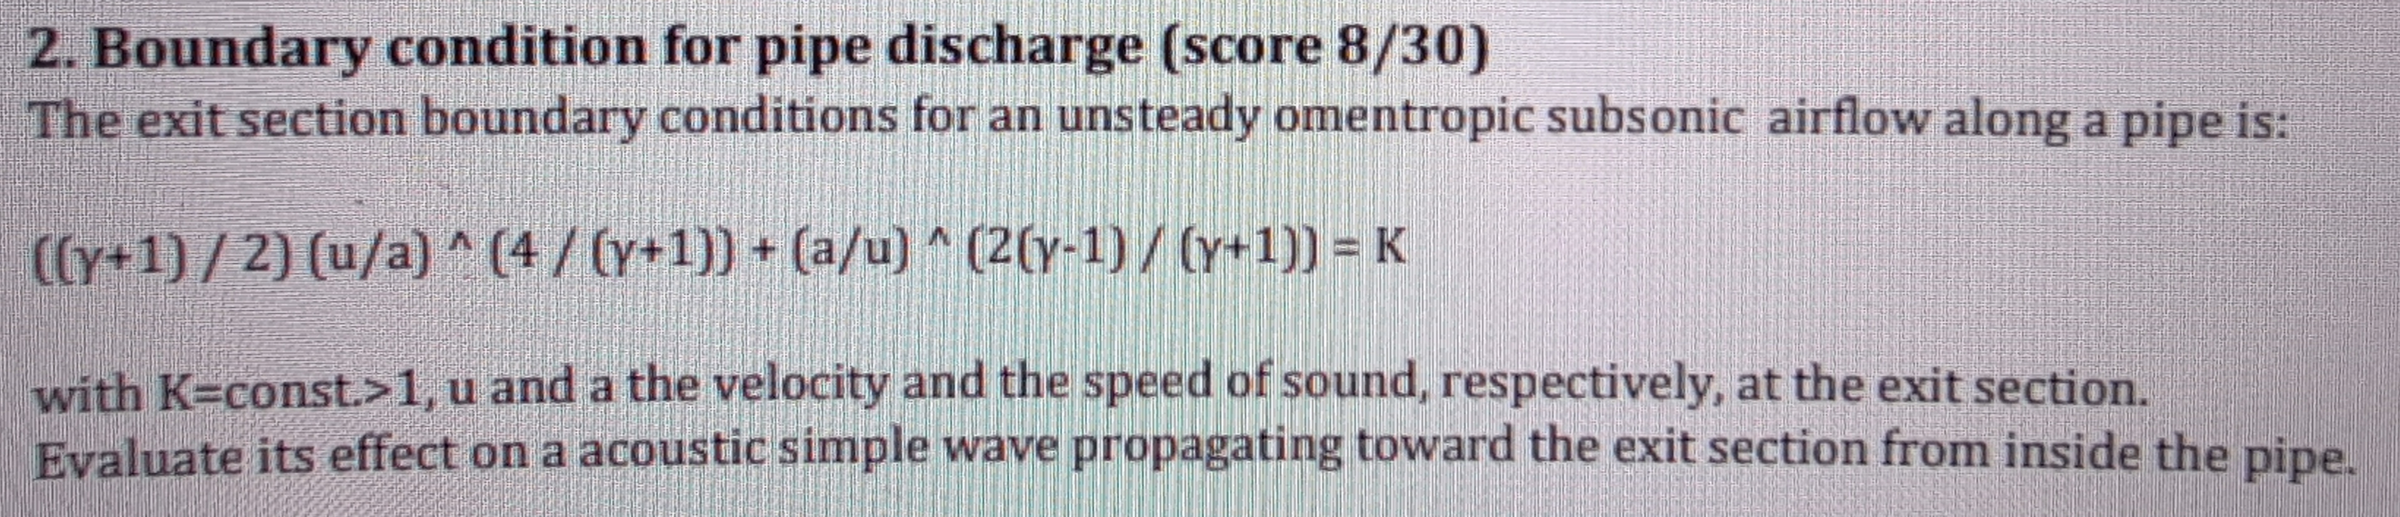
\includegraphics[width=0.85\textwidth]{originale.png}
  \caption{Testo originale dell'esercizio.}
\end{figure}
La traccia coincide con l'esercizio 2 della prova del 13/02/2023 (B70-E02 del catalogo). È affine B67-E02
(14/01/2022), dove all'uscita si impone il Mach iniziale e il disturbo incidente è un'onda di entropia.

%==============================================================================
\section{Lettura del testo e dati}
Il primo membro dipende da $u$ e $a$ solo attraverso il loro rapporto: con $M=u/a$
\[
  f(M)=\frac{\gamma+1}{2}M^{4/(\gamma+1)}+M^{-2(\gamma-1)/(\gamma+1)}=K .
\]
La condizione quindi \textbf{fissa il numero di Mach nella sezione d'uscita}, qualunque cosa succeda a $p$, $\rho$,
$u$ e $a$ separatamente: lo dimostro nel calcolo.

Il testo dà altre informazioni. Si tratta di uno \emph{scarico} (\emph{discharge}): il gas esce, $u>0$ verso la
sezione d'uscita, che pongo all'estremo destro ($x$ verso l'esterno). Il flusso è \emph{omoentropico} e
\emph{subsonico}, $0<M<1$. Il gas è aria, $\gamma=1{,}4$, quindi $\delta=(\gamma-1)/2=0{,}2$. L'onda che arriva
``dall'interno'' è un'onda semplice di piccola ampiezza (acustica), e può essere una compressione o
un'espansione. Non ci sono dati numerici: svolgo il problema in forma letterale e uso un esempio numerico solo
per i diagrammi.

\begin{table}[H]
  \centering
  \begin{tabular}{lll}
    \toprule
    Grandezza & Valore & Note \\
    \midrule
    $\gamma$ & \num{1.4} & aria, $\delta=0{,}2$ \\
    $K$ & costante $>1$ & assegnata, nessun valore numerico \\
    $0<M<1$ & & uscita subsonica, $u>0$ (scarico) \\
    onda incidente & semplice, acustica & dall'interno verso l'uscita \\
    esempio (solo diagrammi) & $\Me=0{,}3$, $p_0=a_0=1$ & $p_1/p_0=1{,}1$ e $0{,}9$ \\
    \bottomrule
  \end{tabular}
  \caption{Dati del problema.}
\end{table}

%==============================================================================
\section{Modello e ipotesi}
\begin{itemize}
  \item \textbf{Eulero 1D instazionario} nel condotto: la sezione è costante e le onde acustiche hanno lunghezza
        molto maggiore del diametro, quindi sono piane. Il gas è perfetto, non viscoso e adiabatico.
  \item \textbf{Omoentropico}, come dice il testo: l'entropia è uniforme, non ci sono onde di entropia e gli
        invarianti di Riemann $\Ru=a-\delta u$ (costante lungo le $\uma$) e $\Rd=a+\delta u$ (costante lungo le
        $\upa$) valgono ovunque. Lo stato è descritto da $a$ e $u$: $p$ e $\rho$ seguono dalle isentropiche.
  \item \textbf{Onda acustica}: l'ampiezza è piccola, quindi l'onda resta isentropica. Una compressione si
        irripidisce, ma la distanza di formazione dell'urto è grande rispetto al tratto che percorre fino
        all'uscita. Le relazioni fra $a$ e $u$ che ricavo sono esatte per qualunque onda continua; le relazioni in
        pressione le linearizzo (acustica).
  \item La condizione vale \textbf{in ogni istante} nella sezione d'uscita: il dispositivo che la realizza (per
        esempio un restringimento strozzato) è corto rispetto alla lunghezza d'onda e risponde in modo
        quasi stazionario.
\end{itemize}

%==============================================================================
\section{Analisi qualitativa}
\textbf{Quante condizioni.} Nella sezione d'uscita, con $0<u<a$, le caratteristiche $u$ e $\upa$ arrivano
dall'interno e escono dal dominio, mentre solo la $\uma$ ($u-a<0$) entra nel condotto. Serve quindi
\textbf{una} condizione, e la traccia ne dà una sola: il problema è ben posto. Il gas è omoentropico, quindi la
$u$ non porta informazioni: all'uscita arriva dall'interno solo $\Rd$, e la condizione deve fissare l'invariante
entrante $\Ru$.

\textbf{Quale onda arriva.} Con $u>0$ e flusso subsonico, un'onda $\uma$ si allontana dall'uscita ($u-a<0$).
L'onda che ``si propaga verso l'uscita dall'interno'' è quindi un'\textbf{onda semplice $\upa$}: al suo interno
$\Ru$ è uniforme e varia $\Rd$. Arrivata all'uscita, l'onda cambia $\Rd$ nella sezione. La condizione lega $\Ru$ a
$\Rd$, quindi cambia anche $\Ru$: nasce un'\textbf{onda riflessa $\uma$} che risale il condotto.

\textbf{Che natura mi aspetto.} Una compressione incidente fa crescere $a$ e $u$, con $\Delta u=\Delta a/\delta$.
Se l'uscita la lasciasse passare così, sarebbe $\Delta u/u=(\Delta a/a)/(\delta M)\gg\Delta a/a$, perché
$\delta M<0{,}2$. Con $M$ fissato, invece, $u$ può crescere solo nella stessa proporzione di $a$: l'uscita
\textbf{frena} il gas, come una parete parziale. Mi aspetto quindi una riflessa della \textbf{stessa natura}
dell'incidente, più debole, in un caso intermedio fra la parete ($u$ imposta, riflessione con la stessa natura) e
l'estremo aperto ($p$ imposta, riflessione con natura opposta).

%==============================================================================
\section{Topologia del campo}
Il campo nel piano $x$--$t$ vicino all'uscita (fig.~\ref{fig:xt}) ha queste regioni:
\begin{itemize}
  \item \textbf{0}: flusso iniziale uniforme, subsonico, che soddisfa già la condizione ($u_0=\Me a_0$);
  \item \textbf{onda incidente $\upa$}: onda semplice, a $\Ru=R_{1,0}$ uniforme, fra la testa (che si propaga a
        $u_0+a_0$ nello stato 0) e la coda;
  \item \textbf{1}: stato uniforme dietro l'incidente, a $R_{1,1}=R_{1,0}$;
  \item \textbf{Z}: zona d'interazione a due famiglie, a ridosso dell'uscita, fra l'istante in cui arriva la testa
        dell'incidente e quello in cui arriva la coda. È delimitata dalla testa della riflessa e dalla coda
        dell'incidente, che si incontrano in P;
  \item \textbf{onda riflessa $\uma$}: onda semplice, a $\Rd=R_{2,1}$ uniforme, che risale nello stato 1;
  \item \textbf{2}: stato uniforme all'uscita dopo la riflessione, a $R_{2,2}=R_{2,1}$, che soddisfa la condizione.
\end{itemize}
Per gli stati uniformi tratto le caratteristiche come semirette. La zona Z si potrebbe risolvere con le
compatibilità lungo le due famiglie e con la condizione all'uscita, ma non serve: lungo ogni $\upa$ l'invariante
$\Rd$ arriva all'uscita invariato anche attraversando Z, e la condizione dà nello stesso istante il $\Ru$ che
riparte. All'uscita la relazione fra le due onde vale quindi istante per istante.

%==============================================================================
\section{Calcolo}
\subsection{La condizione impone $M$ costante}
Derivo la condizione rispetto al tempo nella sezione d'uscita:
\[
  \frac{d f}{d t}=f'(M)\,M_t=0,\qquad
  f'(M)=2M^{-(3\gamma-1)/(\gamma+1)}\left[M^2-\frac{\gamma-1}{\gamma+1}\right],\qquad
  M_t=\frac{u_t-M\,a_t}{a}.
\]
Per $M\neq0$ (scarico, $u>0$) e $M\neq M_m=\sqrt{(\gamma-1)/(\gamma+1)}$ resta
\[
  u_t-M\,a_t=0\quad\Longleftrightarrow\quad M_t=0 :
\]
\textbf{il Mach d'uscita è costante}, $M=\Me$, e $\Me$ è una radice di $f(M)=K$.

\textbf{Quali radici.} $f\to\infty$ per $M\to0$ e per $M\to\infty$, e $f'$ si annulla solo in $M_m$, dove $f$ ha il
minimo. Sostituendo $M_m^2=(\gamma-1)/(\gamma+1)$ e raccogliendo $M_m^{-2(\gamma-1)/(\gamma+1)}$:
\[
  f_{min}=M_m^{-2(\gamma-1)/(\gamma+1)}\left[\frac{\gamma+1}{2}M_m^2+1\right]
  =\frac{\gamma+1}{2}\left(\frac{\gamma+1}{\gamma-1}\right)^{(\gamma-1)/(\gamma+1)}\approx1{,}62,
  \qquad M_m\approx0{,}408 .
\]
Inoltre $f(1)=(\gamma+3)/2=2{,}2$. Quindi (fig.~\ref{fig:f}):
\begin{itemize}
  \item $1<K<f_{min}$: nessuno stato d'uscita soddisfa la condizione. Il dato $K>1$ della traccia è necessario
        ($f_{min}>1$ per ogni $\gamma$), ma non sufficiente;
  \item $f_{min}<K<(\gamma+3)/2$: due radici subsoniche, una sotto e una sopra $M_m$;
  \item $K\ge(\gamma+3)/2$: una sola radice subsonica ($\Me<M_m$); l'altra è sonica o supersonica ed è esclusa;
  \item $K=f_{min}$: radice doppia $\Me=M_m$. La forma derivata non dà informazioni ($f'=0$), ma $f$ ha lì un
        minimo stretto: ogni variazione di $M$ darebbe $f>K$, quindi anche in questo caso $M=M_m$ resta fisso.
\end{itemize}
Delle due radici vale quella del flusso iniziale. $M$ varia con continuità e la condizione gli vieta di cambiare,
quindi l'uscita non può passare all'altra radice. Escludo anche $M=1$: con uscita sonica nessuna caratteristica
entra dall'uscita e non si può imporre alcuna condizione.

\subsection{La condizione in termini di invarianti}
Con $u=\Me a$ nella sezione d'uscita ho $\Ru=a-\delta u=a(1-\delta\Me)$ e $\Rd=a+\delta u=a(1+\delta\Me)$, quindi
\[
  \Ru\big|_{uscita}=\Cr\,\Rd\big|_{uscita},\qquad \Cr=\frac{1-\delta\Me}{1+\delta\Me} .
\]
La relazione è \textbf{esatta e lineare}: l'invariante che entra nel condotto è proporzionale a quello che arriva
dall'interno. In ogni istante le incognite all'uscita sono $a$ e $u$. Le equazioni sono due: l'invariante $\Rd$
portato dalla $\upa$ e la condizione. Lo stato all'uscita è quindi determinato senza iterare.

\subsection{Stati 0, 1, 2}
\textbf{Stato 0.} Soddisfa la condizione: $u_0=\Me a_0$, cioè $R_{1,0}=\Cr\,R_{2,0}$.

\textbf{Stato 1} (dietro l'incidente $\upa$). Attraverso l'onda $\upa$ resta $R_{1,1}=R_{1,0}$, mentre $\Rd$ cambia
di $\Delta\Rd=R_{2,1}-R_{2,0}$, che misura l'intensità dell'incidente. Da $a=(\Ru+\Rd)/2$ e $u=(\Rd-\Ru)/(2\delta)$:
\[
  \Delta a_i=a_1-a_0=\tfrac12\Delta\Rd,\qquad \Delta u_i=u_1-u_0=\frac{\Delta a_i}{\delta}.
\]

\textbf{Stato 2} (dietro la riflessa $\uma$, nella sezione d'uscita). Attraverso la riflessa resta
$R_{2,2}=R_{2,1}$, e la condizione dà $R_{1,2}=\Cr\,R_{2,1}$. Sottraggo la relazione dello stato 0 e uso
$R_{1,1}=R_{1,0}$:
\[
  \Delta\Ru=R_{1,2}-R_{1,1}=\Cr\,\Delta\Rd .
\]
Attraverso la riflessa $\Delta a_r=a_2-a_1=\tfrac12\Delta\Ru$ e $\Delta u_r=u_2-u_1=-\Delta a_r/\delta$, quindi
\[
  \boxed{\;\frac{\Delta a_r}{\Delta a_i}=\frac{\Delta\Ru}{\Delta\Rd}=\Cr=\frac{1-\delta\Me}{1+\delta\Me},\qquad
  \frac{\Delta u_r}{\Delta u_i}=-\Cr\;}
\]
con $0<\Cr<1$ per $0<\Me<1$. Nella sezione d'uscita le variazioni complessive sono
\[
  a_2-a_0=(1+\Cr)\,\Delta a_i=\frac{2\,\Delta a_i}{1+\delta\Me},\qquad
  u_2-u_0=(1-\Cr)\,\Delta u_i=\frac{2\delta\Me}{1+\delta\Me}\,\Delta u_i .
\]
Per onde acustiche $\Delta p/p=\frac{2\gamma}{\gamma-1}\Delta a/a$ con lo stesso $p/a$ di riferimento, quindi le
pressioni seguono le $a$:
\[
  \frac{\Delta p_r}{\Delta p_i}\approx\Cr,\qquad p_2-p_0\approx(1+\Cr)\,\Delta p_i .
\]
Con $\Me$ da $0$ a $1$, $\Cr$ scende da $1$ a $(3-\gamma)/(\gamma+1)=2/3$; i valori per l'aria sono in
tab.~\ref{tab:C}.

\begin{table}[H]
  \centering
  \begin{tabular}{cccc}
    \toprule
    $\Me$ & $\Cr=\Delta p_r/\Delta p_i$ & $(p_2-p_0)/\Delta p_i=1+\Cr$ & $(u_2-u_0)/\Delta u_i=1-\Cr$ \\
    \midrule
    0,1 & 0,961 & 1,96 & 0,039 \\
    0,2 & 0,923 & 1,92 & 0,077 \\
    0,3 & 0,887 & 1,89 & 0,113 \\
    0,408 ($M_m$) & 0,849 & 1,85 & 0,151 \\
    0,6 & 0,786 & 1,79 & 0,214 \\
    0,8 & 0,724 & 1,72 & 0,276 \\
    \bottomrule
  \end{tabular}
  \caption{Riflessione all'uscita per l'aria ($\gamma=1{,}4$), in funzione del Mach d'uscita.}
  \label{tab:C}
\end{table}

\subsection{Forma differenziale: i gradienti delle due onde}
Le stesse conclusioni si leggono sui gradienti, scrivendo la condizione in forma differenziale come
$u_t-M a_t=0$. Le relazioni caratteristiche $R_{1t}+(u-a)R_{1x}=0$ e $R_{2t}+(u+a)R_{2x}=0$, con $a=(\Ru+\Rd)/2$ e
$u=(\Rd-\Ru)/(2\delta)$, danno nella sezione d'uscita
\[
  a_t=-\frac{u+a}{2}\,(a+\delta u)_x-\frac{u-a}{2}\,(a-\delta u)_x,\qquad
  u_t=-\frac{u+a}{2\delta}\,(a+\delta u)_x+\frac{u-a}{2\delta}\,(a-\delta u)_x .
\]
Sostituendo in $u_t-Ma_t=0$, con $u=Ma$ e $M\neq1$:
\[
  (a-\delta u)_x=-\frac{(1+M)(1-\delta M)}{(1-M)(1+\delta M)}\,(a+\delta u)_x .
\]
Nell'incidente $\upa$ ($\Ru$ uniforme) $(a+\delta u)_x=2a_{x,i}$. Nella riflessa $\uma$ ($\Rd$ uniforme)
$(a-\delta u)_x=2a_{x,r}$. Quindi
\[
  a_{x,r}=-\frac{1+\Me}{1-\Me}\,\Cr\;a_{x,i}.
\]
Una compressione incidente $\upa$ ha $a_{x,i}<0$, perché il gas compresso sta dietro, a sinistra. Allora
$a_{x,r}>0$: la riflessa $\uma$ ha il gas compresso dietro di sé, a destra, ed è una \textbf{compressione}.
Allo stesso modo un'espansione si riflette come espansione. Il fattore $(1+\Me)/(1-\Me)=(a+u)/(a-u)$, in più
rispetto al rapporto delle ampiezze, è il rapporto delle velocità di propagazione. All'uscita la riflessa ha la
stessa durata dell'incidente, ma risale la corrente più lentamente: nello spazio è più corta e più ripida.

\subsection{Esempio numerico}
Per i diagrammi scelgo $\Me=0{,}3$, a cui corrisponde $K=f(0{,}3)\approx1{,}66$ (l'altra radice subsonica è
$\approx0{,}54$), e quindi $\Cr\approx0{,}887$. Prendo $p_0=a_0=1$, $u_0=0{,}3$ e un'incidente di compressione con
$p_1/p_0=1{,}1$, più ampia di un'onda acustica perché i punti siano leggibili. Con $a_1=a_0(p_1/p_0)^{(\gamma-1)/(2\gamma)}$
e $u_1=u_0+(a_1-a_0)/\delta$:
\[
  a_1\approx1{,}014,\qquad u_1\approx0{,}369 .
\]
Lo stato 2 segue da $R_{2,2}=R_{2,1}$ e da $u_2=\Me a_2$:
\[
  a_2=\frac{R_{2,1}}{1+\delta\Me}\approx1{,}026,\qquad u_2=\Me a_2\approx0{,}308,\qquad
  p_2=p_0\left(\frac{a_2}{a_0}\right)^{2\gamma/(\gamma-1)}\approx1{,}20 .
\]
La riflessa porta la pressione da $1{,}10$ a $\approx1{,}20$. Per confronto, a pari onda incidente:
\begin{itemize}
  \item un'uscita a pressione imposta ($p=p_0$) darebbe $u\approx0{,}437$, con una riflessa di espansione;
  \item un'uscita a velocità imposta ($u=u_0$) darebbe $p\approx1{,}21$.
\end{itemize}
Con un'incidente di espansione $p_1/p_0=0{,}9$ si ottiene $p_2\approx0{,}82$: anche qui la riflessa ha la stessa
natura dell'incidente.

%==============================================================================
\section{Verifiche a posteriori}
\begin{itemize}
  \item Numero di condizioni: all'uscita subsonica entra solo la $\uma$, e la condizione è una: verificata.
  \item Uscita subsonica e riflessa entrante: $M$ resta $\Me<1$, quindi $u_2-a_2=-(1-\Me)a_2<0$ e la riflessa
        risale il condotto: verificata.
  \item Natura della riflessa: $\Delta a_r/\Delta a_i=\Cr>0$, stesso segno; coincide con il segno dei gradienti
        della forma differenziale: verificata.
  \item Condizione nello stato 2: $(u_2-u_0)/(a_2-a_0)=(1-\Cr)/[\delta(1+\Cr)]=\Me$, cioè $\Delta u/u=\Delta a/a$ e
        $M$ resta $\Me$: verificata.
  \item Limite $\Me\to0$: $\Cr\to1$ e $u_2=u_0=0$, cioè la riflessione su parete: verificata.
  \item Coerenza acustica: $\Delta p_r=-\rho a\,\Delta u_r$ (onda $\uma$) con $\Delta p_r=\Cr\Delta p_i$ e
        $\Delta u_r=-\Cr\Delta u_i$, dato che $\Delta p_i=\rho a\,\Delta u_i$ (onda $\upa$): verificata.
  \item Niente vuoto: $a_2=R_{2,1}/(1+\delta\Me)>0$ per qualunque espansione incidente con $R_{2,1}>0$: verificata.
  \item Omoentropia: onde acustiche, nessun urto; la riflessa di compressione è più ripida di $(1+\Me)/(1-\Me)$,
        ma con piccola ampiezza la formazione dell'urto resta lontana: verificata.
  \item Esistenza: la condizione ammette uno stato subsonico solo per $K\ge f_{min}\approx1{,}62$; per
        $1<K<f_{min}$ la traccia non sarebbe realizzabile.
\end{itemize}

%==============================================================================
\section{Risultati}
\begin{table}[H]
  \centering
  \small
  \begin{tabular}{lll}
    \toprule
    Grandezza & Risultato & Esatto/approssimato \\
    \midrule
    effetto della condizione & $M=\Me$ costante, radice di $f(M)=K$ & esatto \\
    esistenza & $K\ge f_{min}\approx1{,}62$; due radici se $K<2{,}2$ & esatto \\
    condizione sugli invarianti & $\Ru=\Cr\Rd$, $\Cr=(1-\delta\Me)/(1+\delta\Me)$ & esatto \\
    onda riflessa & $\uma$, \textbf{stessa natura} dell'incidente & esatto \\
    ampiezza in $a$ e $u$ & $\Delta a_r=\Cr\Delta a_i$, $\Delta u_r=-\Cr\Delta u_i$ & esatto \\
    ampiezza in $p$ & $\Delta p_r\approx\Cr\Delta p_i$, $p_2-p_0\approx(1+\Cr)\Delta p_i$ & acustico \\
    velocità all'uscita & $u_2-u_0=2\delta\Me\,\Delta u_i/(1+\delta\Me)$ & esatto \\
    gradienti & $a_{x,r}=-\Cr(1+\Me)/(1-\Me)\,a_{x,i}$ & esatto \\
    campo di $\Cr$ (aria) & da $1$ ($\Me\to0$) a $2/3$ ($\Me\to1$) & esatto \\
    \bottomrule
  \end{tabular}
  \caption{Risultati.}
\end{table}

%==============================================================================
\section{Rappresentazioni}
\begin{figure}[H]
  \centering
  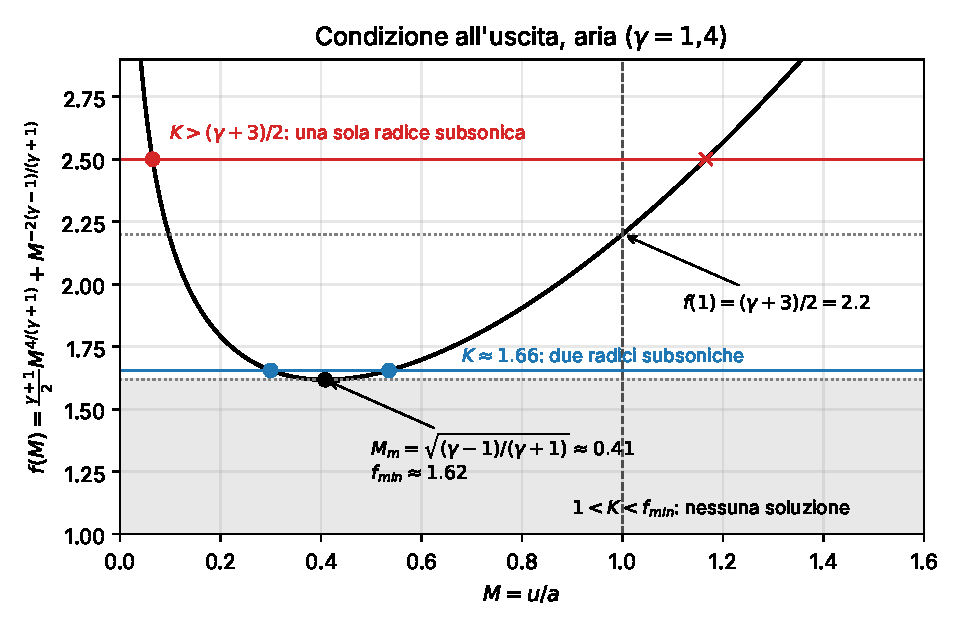
\includegraphics[width=0.72\textwidth]{funzione_K.pdf}
  \caption{La funzione $f(M)$ della condizione per l'aria: minimo in $M_m$, valore sonico $f(1)$, radici per due
  valori di $K$.}
  \label{fig:f}
\end{figure}
La fig.~\ref{fig:f} mostra perché la condizione equivale a $M=\Me$: a $K$ fissato la retta orizzontale taglia la
curva in punti isolati. Fra $f_{min}$ e $2{,}2$ ci sono due radici subsoniche ai lati di $M_m$ (esempio
$K\approx1{,}66$: $\Me=0{,}3$ e $\approx0{,}54$). Sopra $2{,}2$ resta una sola radice subsonica, piccola (per $K=2{,}5$,
$\Me\approx0{,}065$), perché l'altra è supersonica. Sotto $f_{min}$ non ci sono soluzioni.

\begin{figure}[H]
  \centering
  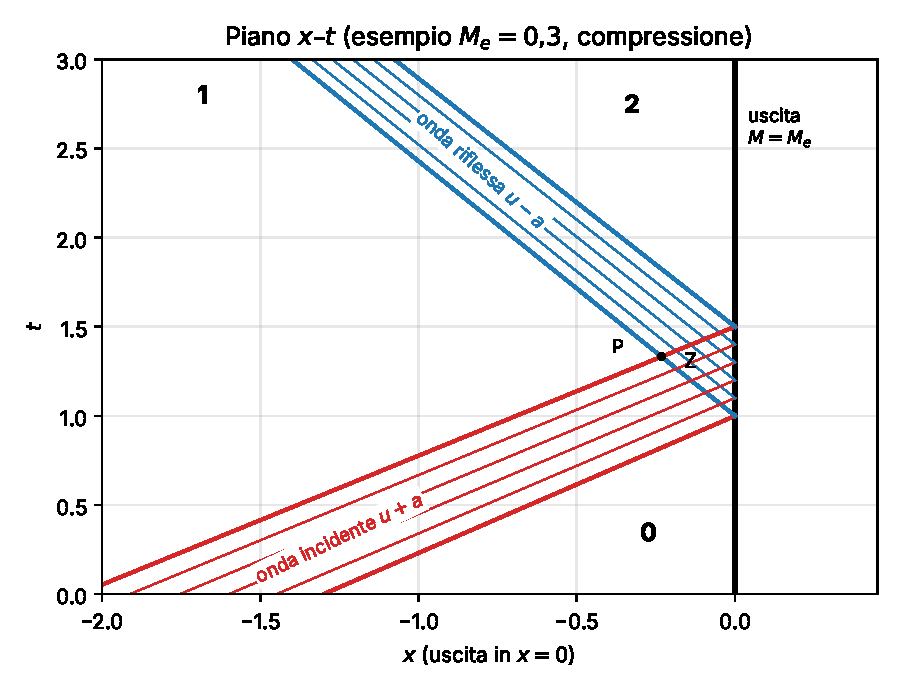
\includegraphics[width=0.68\textwidth]{xt.pdf}
  \caption{Piano $x$--$t$ vicino all'uscita (esempio $\Me=0{,}3$, compressione incidente), con caratteristiche
  rettilinee: stati 0, 1, 2, zona d'interazione Z.}
  \label{fig:xt}
\end{figure}
Nella fig.~\ref{fig:xt} l'incidente $\upa$ (rosso) arriva all'uscita fra $t=1$ e $t=1{,}5$. Ogni sua
caratteristica genera nello stesso istante una caratteristica $\uma$ della riflessa (blu). Le $\upa$ dell'incidente
sono più veloci delle $\uma$ della riflessa ($a+u>a-u$), quindi più vicine all'orizzontale: la riflessa occupa
nello spazio un tratto più corto. Le due onde si sovrappongono nel triangolo Z, chiuso dal punto P; oltre P la riflessa risale nello stato 1,
come onda semplice.

\begin{figure}[H]
  \centering
  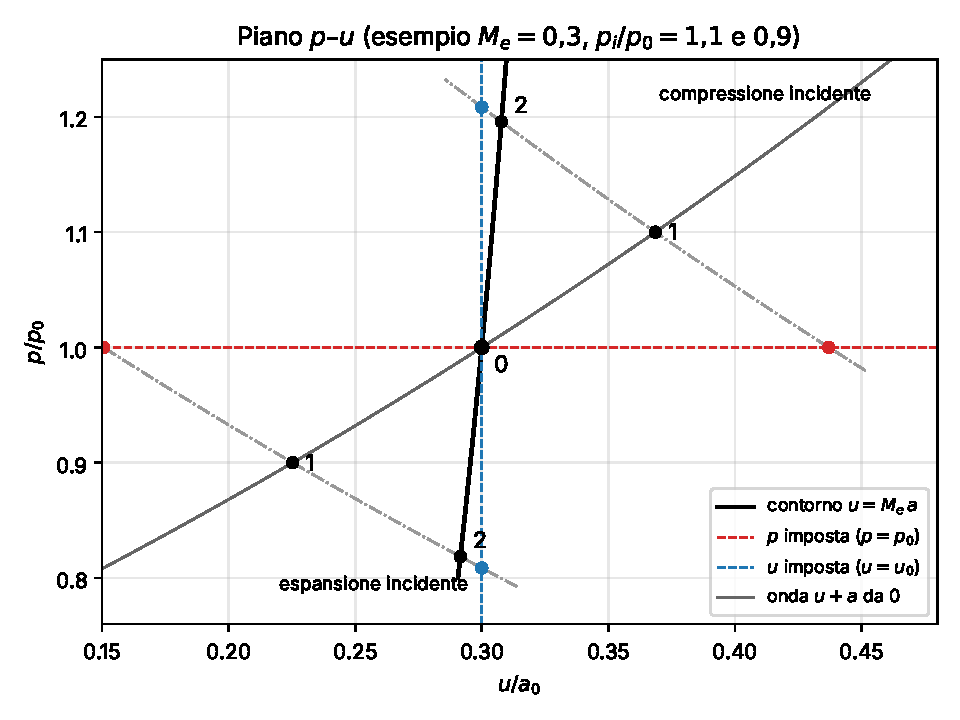
\includegraphics[width=0.72\textwidth]{pu.pdf}
  \caption{Piano $p$--$u$ (esempio $\Me=0{,}3$): curva del contorno $u=\Me a$ e confronto con pressione e velocità
  imposte, per un'incidente di compressione ($p_1/p_0=1{,}1$) e di espansione ($0{,}9$).}
  \label{fig:pu}
\end{figure}
Nella fig.~\ref{fig:pu}, lo stato 1 sta sulla curva dell'onda $\upa$ uscente da 0. Lo stato 2 è l'intersezione
della curva della riflessa $\uma$ uscente da 1 (tratto-punto) con la curva del contorno $u=\Me a$, quasi verticale:
$u$ cambia poco e $p$ cambia molto, come su una parete. L'intersezione cade dalla stessa parte di 1 rispetto a 0,
cioè sopra 1 per la compressione e sotto 1 per l'espansione: la riflessa ha la stessa natura dell'incidente. I
punti colorati sono le intersezioni con $p=p_0$ (rosso, natura opposta) e con $u=u_0$ (blu, parete). Lo stato 2
cade vicino a quello di velocità imposta, a conferma che l'uscita a Mach imposto si comporta quasi come
un'estremità chiusa. Le pressioni coprono un intervallo stretto, quindi basta la scala lineare.

\begin{figure}[H]
  \centering
  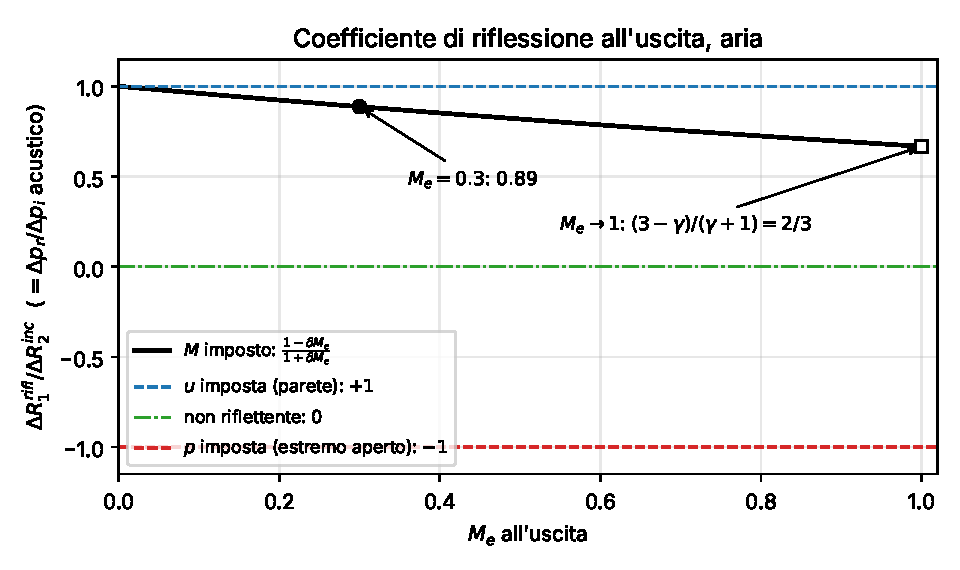
\includegraphics[width=0.72\textwidth]{coeff_riflessione.pdf}
  \caption{Coefficiente di riflessione all'uscita in funzione di $\Me$ (aria), confrontato con velocità imposta,
  contorno non riflettente e pressione imposta.}
  \label{fig:C}
\end{figure}
La fig.~\ref{fig:C} riassume la risposta. Con Mach imposto, $\Cr$ resta fra $2/3$ e $1$ per tutte le uscite
subsoniche, lontano dal contorno non riflettente ($0$) e dall'estremo aperto ($-1$).

%==============================================================================
\section{Discussione fisica}
\textbf{Che cosa rappresenta la condizione.} Fissare il Mach d'uscita è ciò che fa, per esempio, un restringimento
o un ugello strozzato allo sbocco: il rapporto fra la sezione del condotto e quella critica fissa $\Me$ con la
legge delle aree, come nello svuotamento di un tubo da un orifizio. Il rapporto $u/a$ è bloccato, mentre $p$, $\rho$,
$a$ e $u$ seguono le onde.

\textbf{Perché la stessa natura.} Il confronto con gli altri contorni si fa scrivendo all'uscita una relazione
lineare $\Delta u=k\,\Delta a$. Da $\Delta\Ru=\Delta a-\delta\Delta u$ e $\Delta\Rd=\Delta a+\delta\Delta u$ segue
$\Cr=(1-\delta k)/(1+\delta k)$. Con velocità imposta ($k=0$) si ha $\Cr=1$; con pressione imposta
($k\to\infty$), $\Cr=-1$. Il contorno non riflettente ($\Cr=0$) richiederebbe $k=1/\delta$, cioè $\Ru$ costante. Il Mach
imposto ha $k=\Me$, e poiché $\Me<1<1/\delta$ la riflessione ha sempre la stessa natura dell'incidente e un'ampiezza
almeno pari a $2/3$ di essa. È un'estremità ``quasi chiusa'', tanto più chiusa quanto più basso è $\Me$.

\textbf{Che cosa esce.} La parte di perturbazione che non si riflette esce come variazione di portata. Da
$\dot m\propto\rho a\Me\propto a^{(\gamma+1)/(\gamma-1)}$ si ha
$\Delta\dot m/\dot m=\frac{\gamma+1}{\gamma-1}\Delta a_2/a=\frac{\gamma+1}{2\gamma}\Delta p_2/p$: la portata cresce con
la pressione, come in un ugello strozzato, ma la velocità d'uscita cambia poco.

\textbf{Conseguenze.} Se il condotto è chiuso all'altro estremo, un disturbo rimbalza fra la parete (che lo
riflette intero) e l'uscita (che ne trattiene la frazione $\Cr$). Ogni andata e ritorno perde solo
$1-\Cr=2\delta\Me/(1+\delta\Me)$ dell'ampiezza in $\Ru$, $\Rd$: a basso $\Me$ lo smorzamento è lento e il condotto
può risuonare. Inoltre la riflessa di compressione è più ripida dell'incidente del fattore $(1+\Me)/(1-\Me)$. Per
ampiezze non piccole degenera in urto prima dell'incidente, e da lì il modello omoentropico non vale più.

\textbf{Limiti del modello.} Il risultato vale finché la condizione resta verificata in ogni istante, cioè per
lunghezze d'onda grandi rispetto al dispositivo d'uscita, e finché il flusso resta subsonico. Se un'espansione
molto forte portasse l'uscita a $M=1$, nessuna caratteristica entrerebbe più dall'uscita e la condizione non
andrebbe più imposta.

\end{document}
